\documentclass[letterpaper,12pt]{article}
\usepackage[margin=.65in,top=.72in,bottom=.62in,headheight=16pt,headsep=15pt,footskip=19pt]{geometry}
\usepackage[T1]{fontenc}
\usepackage{lmodern,tikz,fancyhdr}\pdfmapfile{+lm.map}
\usetikzlibrary{arrows.meta,shapes.geometric}
\pagestyle{fancy}\fancyhf{}\renewcommand{\headrulewidth}{0pt}\renewcommand{\footrulewidth}{0pt}
\setlength{\parindent}{0pt}\setlength{\parskip}{0pt}
\fancyhead[L]{\small Week 43 / Shuffling picture cards / Grades 4--5}
\fancyfoot[L]{\footnotesize Bellingham Math Circle / Week 43 / W43-grades-4-5-v2}\fancyfoot[R]{\footnotesize\thepage}
\begin{document}
\noindent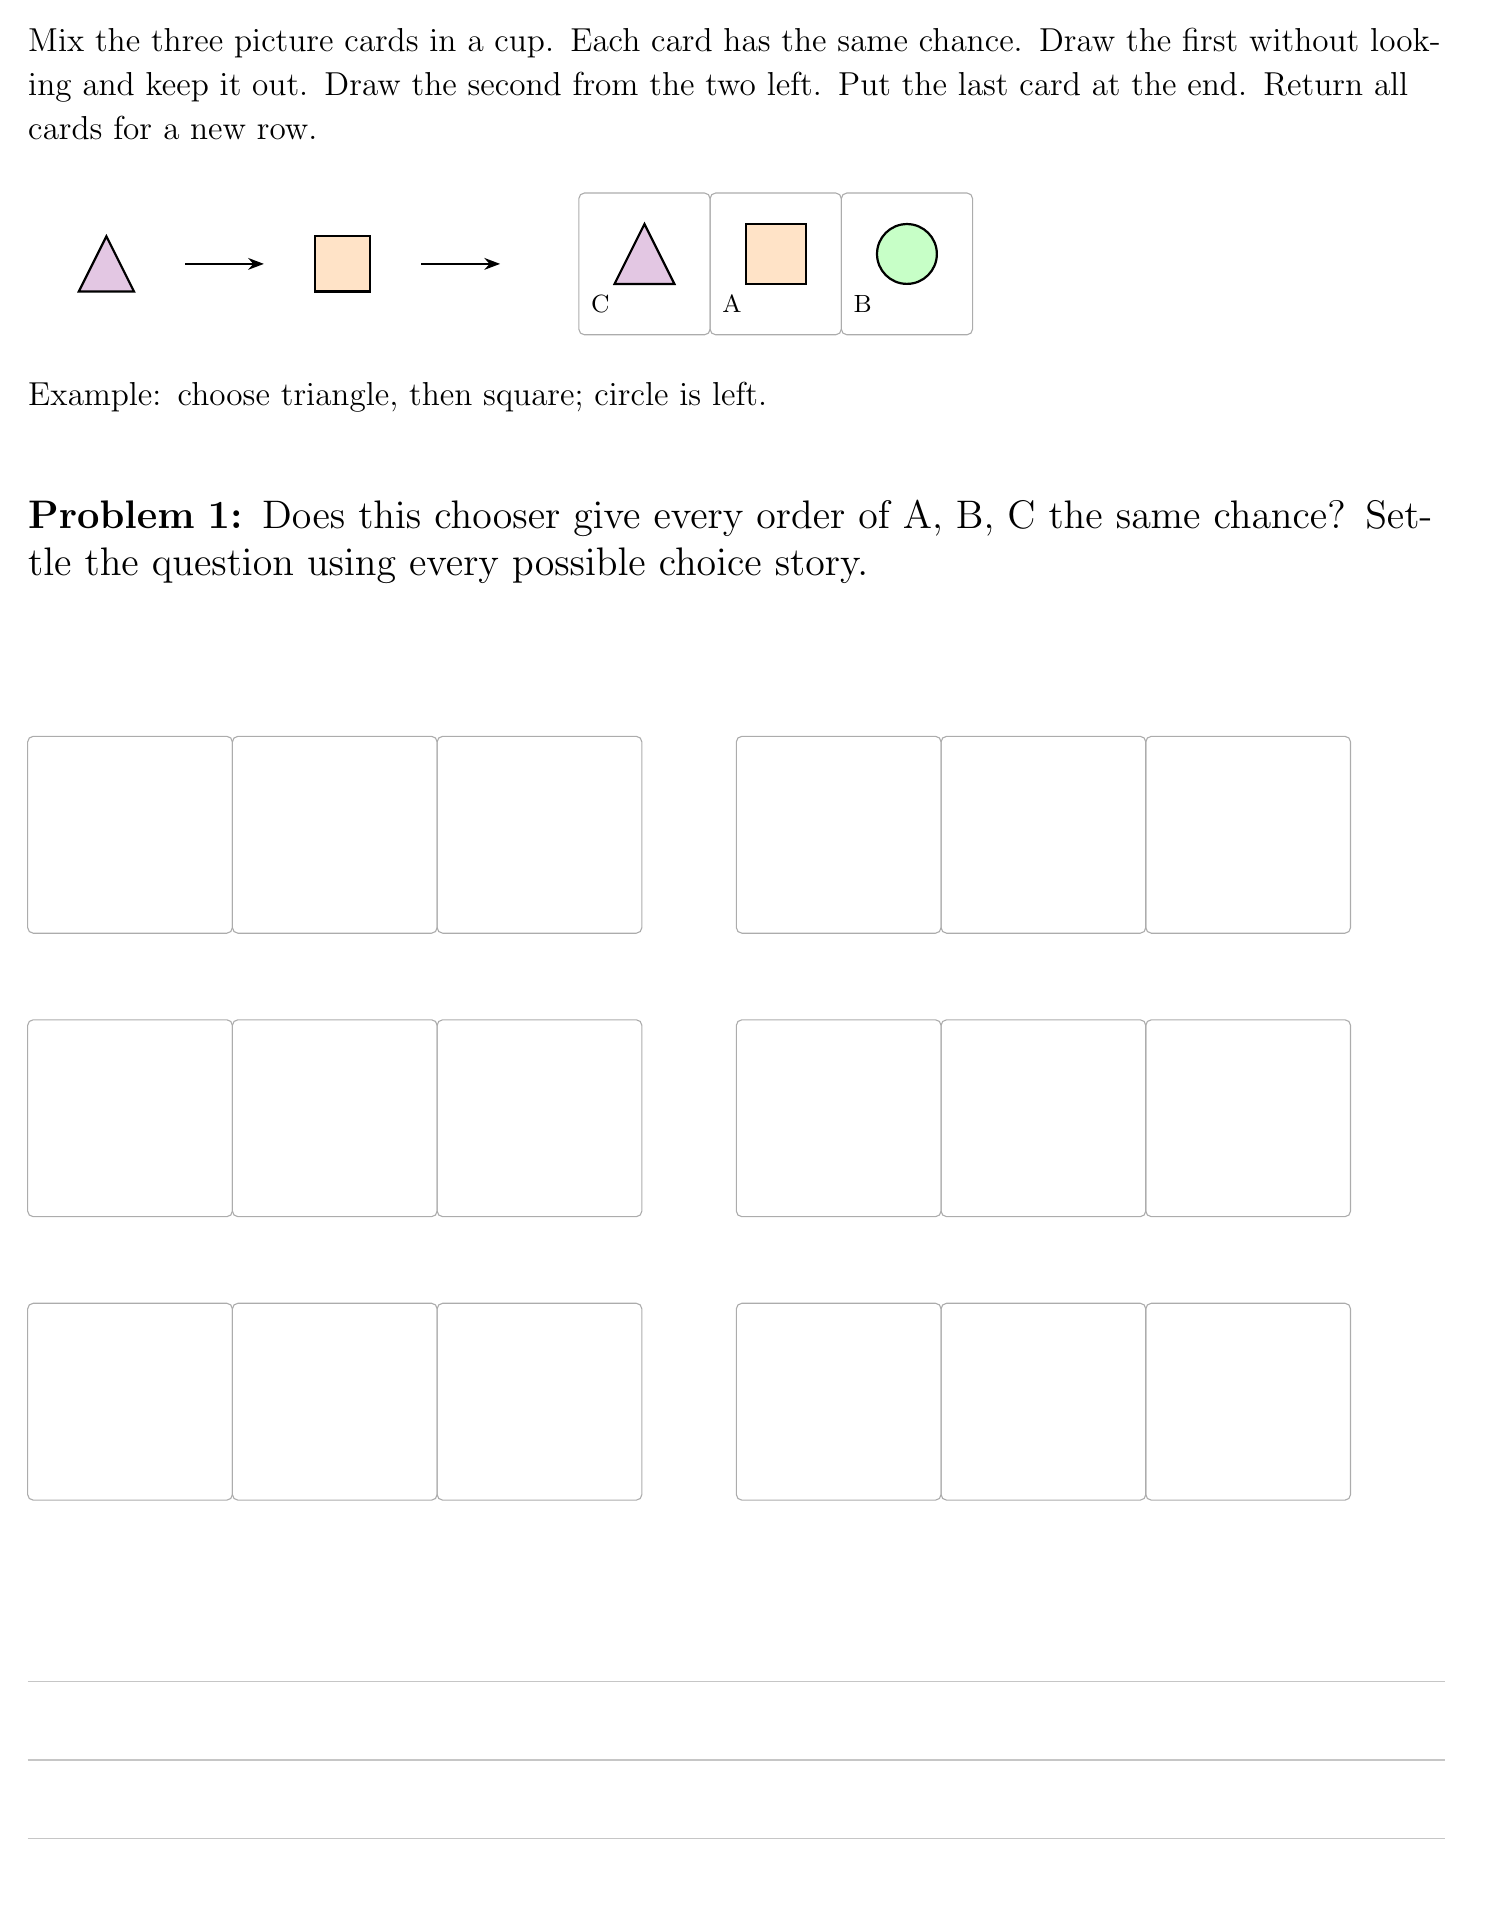
\begin{tikzpicture}[x=1cm,y=1cm]\path[use as bounding box] (0,0) rectangle (18.2,-23.6);
\node[anchor=north west,text width=18cm,inner sep=0pt,font=\fontsize{13}{16}\selectfont] at (0,0) {Mix the three picture cards in a cup. Each card has the same chance. Draw the first without looking and keep it out. Draw the second from the two left. Put the last card at the end. Return all cards for a new row.};
\draw[fill=violet!22,line width=.8pt] (1,-2.65) -- (1.35,-3.35) -- (0.65,-3.35) -- cycle;
\draw[-{Stealth[length=2mm]},line width=.8pt] (2,-3) -- (3,-3) node[midway,above,font=\small] {};
\draw[fill=orange!22,line width=.8pt] (3.65,-3.35) rectangle (4.35,-2.65);
\draw[-{Stealth[length=2mm]},line width=.8pt] (5,-3) -- (6,-3) node[midway,above,font=\small] {};
\draw[gray!65,rounded corners=2pt] (7.0,-2.1) rectangle (8.666666666666666,-3.9000000000000004);
\draw[fill=violet!22,line width=.8pt] (7.833333333333333,-2.494) -- (8.213333333333333,-3.254) -- (7.453333333333333,-3.254) -- cycle;
\node[anchor=north west,text width=1.4666666666666668cm,inner sep=0pt,font=\fontsize{9}{12}\selectfont] at (7.15,-3.396) {C};
\draw[gray!65,rounded corners=2pt] (8.666666666666666,-2.1) rectangle (10.333333333333332,-3.9000000000000004);
\draw[fill=orange!22,line width=.8pt] (9.12,-3.254) rectangle (9.88,-2.494);
\node[anchor=north west,text width=1.4666666666666668cm,inner sep=0pt,font=\fontsize{9}{12}\selectfont] at (8.816666666666666,-3.396) {A};
\draw[gray!65,rounded corners=2pt] (10.333333333333334,-2.1) rectangle (12.0,-3.9000000000000004);
\draw[fill=green!22,line width=.8pt] (11.166666666666668,-2.874) circle (0.38);
\node[anchor=north west,text width=1.4666666666666668cm,inner sep=0pt,font=\fontsize{9}{12}\selectfont] at (10.483333333333334,-3.396) {B};
\node[anchor=north west,text width=18cm,inner sep=0pt,font=\fontsize{12}{15}\selectfont] at (0,-4.5) {Example: choose triangle, then square; circle is left.};
\node[anchor=north west,text width=18cm,inner sep=0pt,font=\fontsize{14}{17}\selectfont] at (0,-6) {\textbf{Problem 1:} Does this chooser give every order of A, B, C the same chance? Settle the question using every possible choice story.};
\draw[gray!65,rounded corners=2pt] (0.0,-9.0) rectangle (2.6,-11.5);
\draw[gray!65,rounded corners=2pt] (2.6,-9.0) rectangle (5.2,-11.5);
\draw[gray!65,rounded corners=2pt] (5.2,-9.0) rectangle (7.800000000000001,-11.5);
\draw[gray!65,rounded corners=2pt] (9.0,-9.0) rectangle (11.6,-11.5);
\draw[gray!65,rounded corners=2pt] (11.6,-9.0) rectangle (14.2,-11.5);
\draw[gray!65,rounded corners=2pt] (14.2,-9.0) rectangle (16.8,-11.5);
\draw[gray!65,rounded corners=2pt] (0.0,-12.6) rectangle (2.6,-15.1);
\draw[gray!65,rounded corners=2pt] (2.6,-12.6) rectangle (5.2,-15.1);
\draw[gray!65,rounded corners=2pt] (5.2,-12.6) rectangle (7.800000000000001,-15.1);
\draw[gray!65,rounded corners=2pt] (9.0,-12.6) rectangle (11.6,-15.1);
\draw[gray!65,rounded corners=2pt] (11.6,-12.6) rectangle (14.2,-15.1);
\draw[gray!65,rounded corners=2pt] (14.2,-12.6) rectangle (16.8,-15.1);
\draw[gray!65,rounded corners=2pt] (0.0,-16.2) rectangle (2.6,-18.7);
\draw[gray!65,rounded corners=2pt] (2.6,-16.2) rectangle (5.2,-18.7);
\draw[gray!65,rounded corners=2pt] (5.2,-16.2) rectangle (7.800000000000001,-18.7);
\draw[gray!65,rounded corners=2pt] (9.0,-16.2) rectangle (11.6,-18.7);
\draw[gray!65,rounded corners=2pt] (11.6,-16.2) rectangle (14.2,-18.7);
\draw[gray!65,rounded corners=2pt] (14.2,-16.2) rectangle (16.8,-18.7);
\draw[gray!45] (0,-21) -- (18,-21);
\draw[gray!45] (0,-22) -- (18,-22);
\draw[gray!45] (0,-23) -- (18,-23);
\end{tikzpicture}
\newpage
\noindent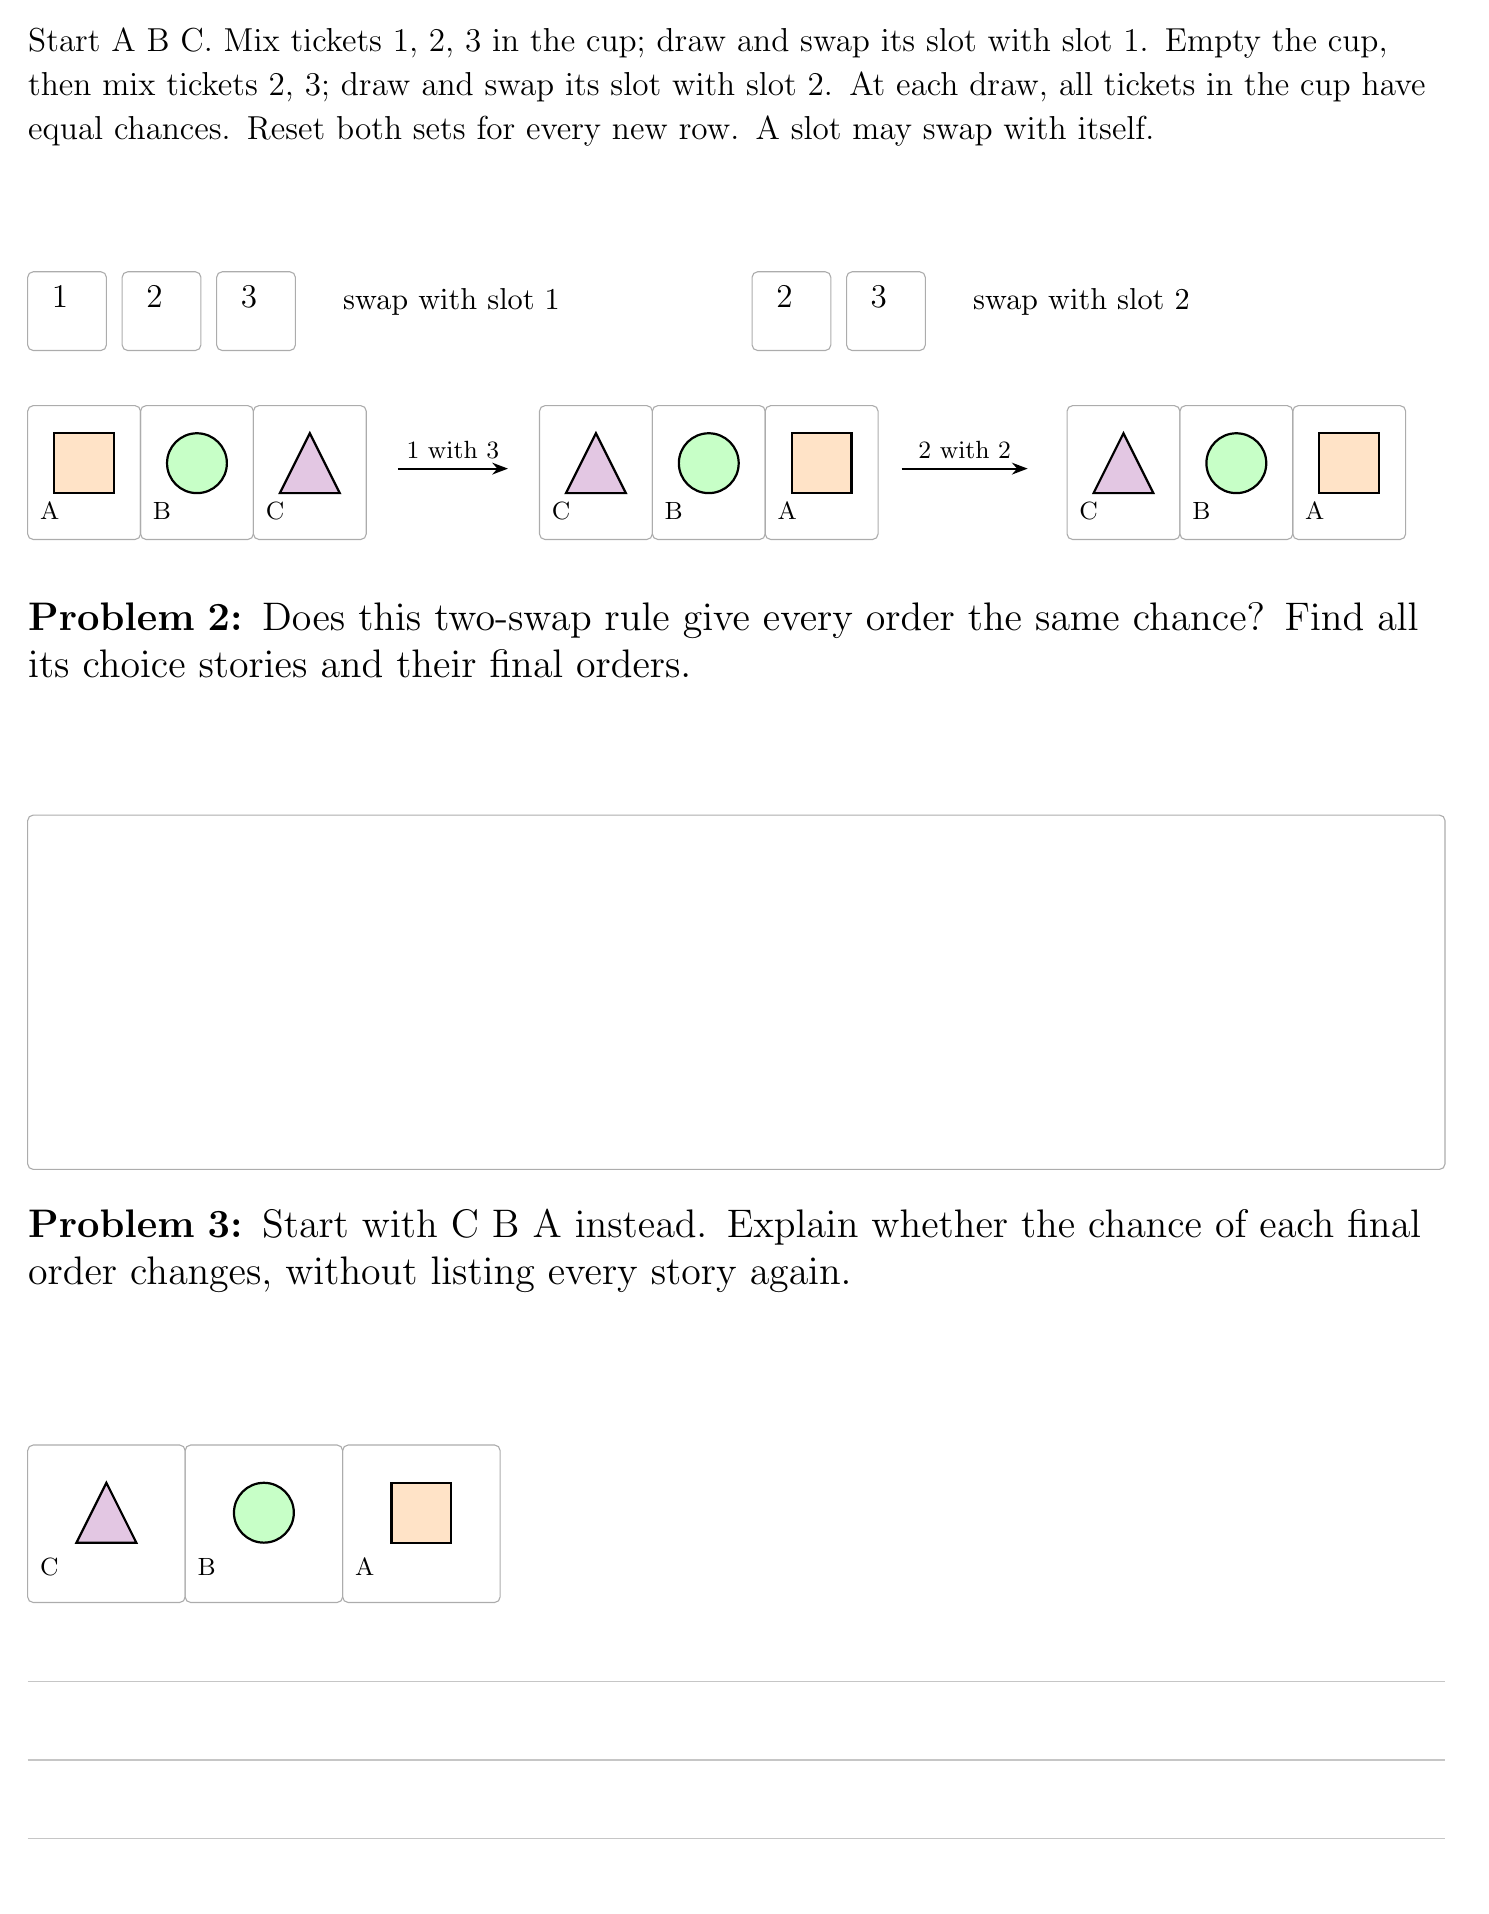
\begin{tikzpicture}[x=1cm,y=1cm]\path[use as bounding box] (0,0) rectangle (18.2,-23.6);
\node[anchor=north west,text width=18cm,inner sep=0pt,font=\fontsize{13}{16}\selectfont] at (0,0) {Start A B C. Mix tickets 1, 2, 3 in the cup; draw and swap its slot with slot 1. Empty the cup, then mix tickets 2, 3; draw and swap its slot with slot 2. At each draw, all tickets in the cup have equal chances. Reset both sets for every new row. A slot may swap with itself.};
\draw[gray!65,rounded corners=2pt] (0.0,-3.1) rectangle (1.0,-4.1);
\node[anchor=north west,text width=0.5cm,inner sep=0pt,font=\fontsize{13}{16}\selectfont] at (0.3,-3.27) {1};
\draw[gray!65,rounded corners=2pt] (1.2,-3.1) rectangle (2.2,-4.1);
\node[anchor=north west,text width=0.5cm,inner sep=0pt,font=\fontsize{13}{16}\selectfont] at (1.5,-3.27) {2};
\draw[gray!65,rounded corners=2pt] (2.4,-3.1) rectangle (3.4,-4.1);
\node[anchor=north west,text width=0.5cm,inner sep=0pt,font=\fontsize{13}{16}\selectfont] at (2.6999999999999997,-3.27) {3};
\node[anchor=north west,text width=5cm,inner sep=0pt,font=\fontsize{11}{14}\selectfont] at (4,-3.3) {swap with slot 1};
\draw[gray!65,rounded corners=2pt] (9.2,-3.1) rectangle (10.2,-4.1);
\node[anchor=north west,text width=0.5cm,inner sep=0pt,font=\fontsize{13}{16}\selectfont] at (9.5,-3.27) {2};
\draw[gray!65,rounded corners=2pt] (10.399999999999999,-3.1) rectangle (11.399999999999999,-4.1);
\node[anchor=north west,text width=0.5cm,inner sep=0pt,font=\fontsize{13}{16}\selectfont] at (10.7,-3.27) {3};
\node[anchor=north west,text width=6cm,inner sep=0pt,font=\fontsize{11}{14}\selectfont] at (12,-3.3) {swap with slot 2};
\draw[gray!65,rounded corners=2pt] (0.0,-4.8) rectangle (1.4333333333333333,-6.5);
\draw[fill=orange!22,line width=.8pt] (0.33666666666666667,-5.911) rectangle (1.0966666666666667,-5.151);
\node[anchor=north west,text width=1.2333333333333334cm,inner sep=0pt,font=\fontsize{9}{12}\selectfont] at (0.15,-6.024) {A};
\draw[gray!65,rounded corners=2pt] (1.4333333333333333,-4.8) rectangle (2.8666666666666667,-6.5);
\draw[fill=green!22,line width=.8pt] (2.15,-5.531) circle (0.38);
\node[anchor=north west,text width=1.2333333333333334cm,inner sep=0pt,font=\fontsize{9}{12}\selectfont] at (1.5833333333333333,-6.024) {B};
\draw[gray!65,rounded corners=2pt] (2.8666666666666667,-4.8) rectangle (4.3,-6.5);
\draw[fill=violet!22,line width=.8pt] (3.5833333333333335,-5.151) -- (3.9633333333333334,-5.911) -- (3.2033333333333336,-5.911) -- cycle;
\node[anchor=north west,text width=1.2333333333333334cm,inner sep=0pt,font=\fontsize{9}{12}\selectfont] at (3.0166666666666666,-6.024) {C};
\draw[-{Stealth[length=2mm]},line width=.8pt] (4.7,-5.6) -- (6.1,-5.6) node[midway,above,font=\small] {1 with 3};
\draw[gray!65,rounded corners=2pt] (6.5,-4.8) rectangle (7.933333333333334,-6.5);
\draw[fill=violet!22,line width=.8pt] (7.216666666666667,-5.151) -- (7.596666666666667,-5.911) -- (6.836666666666667,-5.911) -- cycle;
\node[anchor=north west,text width=1.2333333333333334cm,inner sep=0pt,font=\fontsize{9}{12}\selectfont] at (6.65,-6.024) {C};
\draw[gray!65,rounded corners=2pt] (7.933333333333334,-4.8) rectangle (9.366666666666667,-6.5);
\draw[fill=green!22,line width=.8pt] (8.65,-5.531) circle (0.38);
\node[anchor=north west,text width=1.2333333333333334cm,inner sep=0pt,font=\fontsize{9}{12}\selectfont] at (8.083333333333334,-6.024) {B};
\draw[gray!65,rounded corners=2pt] (9.366666666666667,-4.8) rectangle (10.8,-6.5);
\draw[fill=orange!22,line width=.8pt] (9.703333333333333,-5.911) rectangle (10.463333333333335,-5.151);
\node[anchor=north west,text width=1.2333333333333334cm,inner sep=0pt,font=\fontsize{9}{12}\selectfont] at (9.516666666666667,-6.024) {A};
\draw[-{Stealth[length=2mm]},line width=.8pt] (11.1,-5.6) -- (12.7,-5.6) node[midway,above,font=\small] {2 with 2};
\draw[gray!65,rounded corners=2pt] (13.2,-4.8) rectangle (14.633333333333333,-6.5);
\draw[fill=violet!22,line width=.8pt] (13.916666666666666,-5.151) -- (14.296666666666667,-5.911) -- (13.536666666666665,-5.911) -- cycle;
\node[anchor=north west,text width=1.2333333333333334cm,inner sep=0pt,font=\fontsize{9}{12}\selectfont] at (13.35,-6.024) {C};
\draw[gray!65,rounded corners=2pt] (14.633333333333333,-4.8) rectangle (16.066666666666666,-6.5);
\draw[fill=green!22,line width=.8pt] (15.35,-5.531) circle (0.38);
\node[anchor=north west,text width=1.2333333333333334cm,inner sep=0pt,font=\fontsize{9}{12}\selectfont] at (14.783333333333333,-6.024) {B};
\draw[gray!65,rounded corners=2pt] (16.066666666666666,-4.8) rectangle (17.5,-6.5);
\draw[fill=orange!22,line width=.8pt] (16.403333333333332,-5.911) rectangle (17.16333333333333,-5.151);
\node[anchor=north west,text width=1.2333333333333334cm,inner sep=0pt,font=\fontsize{9}{12}\selectfont] at (16.216666666666665,-6.024) {A};
\node[anchor=north west,text width=18cm,inner sep=0pt,font=\fontsize{14}{17}\selectfont] at (0,-7.3) {\textbf{Problem 2:} Does this two-swap rule give every order the same chance? Find all its choice stories and their final orders.};
\draw[gray!65,rounded corners=2pt] (0,-10) rectangle (18,-14.5);
\node[anchor=north west,text width=18cm,inner sep=0pt,font=\fontsize{14}{17}\selectfont] at (0,-15) {\textbf{Problem 3:} Start with C B A instead. Explain whether the chance of each final order changes, without listing every story again.};
\draw[gray!65,rounded corners=2pt] (0.0,-18) rectangle (2.0,-20);
\draw[fill=violet!22,line width=.8pt] (1.0,-18.48) -- (1.38,-19.24) -- (0.62,-19.24) -- cycle;
\node[anchor=north west,text width=1.8cm,inner sep=0pt,font=\fontsize{9}{12}\selectfont] at (0.15,-19.44) {C};
\draw[gray!65,rounded corners=2pt] (2.0,-18) rectangle (4.0,-20);
\draw[fill=green!22,line width=.8pt] (3.0,-18.86) circle (0.38);
\node[anchor=north west,text width=1.8cm,inner sep=0pt,font=\fontsize{9}{12}\selectfont] at (2.15,-19.44) {B};
\draw[gray!65,rounded corners=2pt] (4.0,-18) rectangle (6.0,-20);
\draw[fill=orange!22,line width=.8pt] (4.62,-19.24) rectangle (5.38,-18.48);
\node[anchor=north west,text width=1.8cm,inner sep=0pt,font=\fontsize{9}{12}\selectfont] at (4.15,-19.44) {A};
\draw[gray!45] (0,-21) -- (18,-21);
\draw[gray!45] (0,-22) -- (18,-22);
\draw[gray!45] (0,-23) -- (18,-23);
\end{tikzpicture}
\newpage
\noindent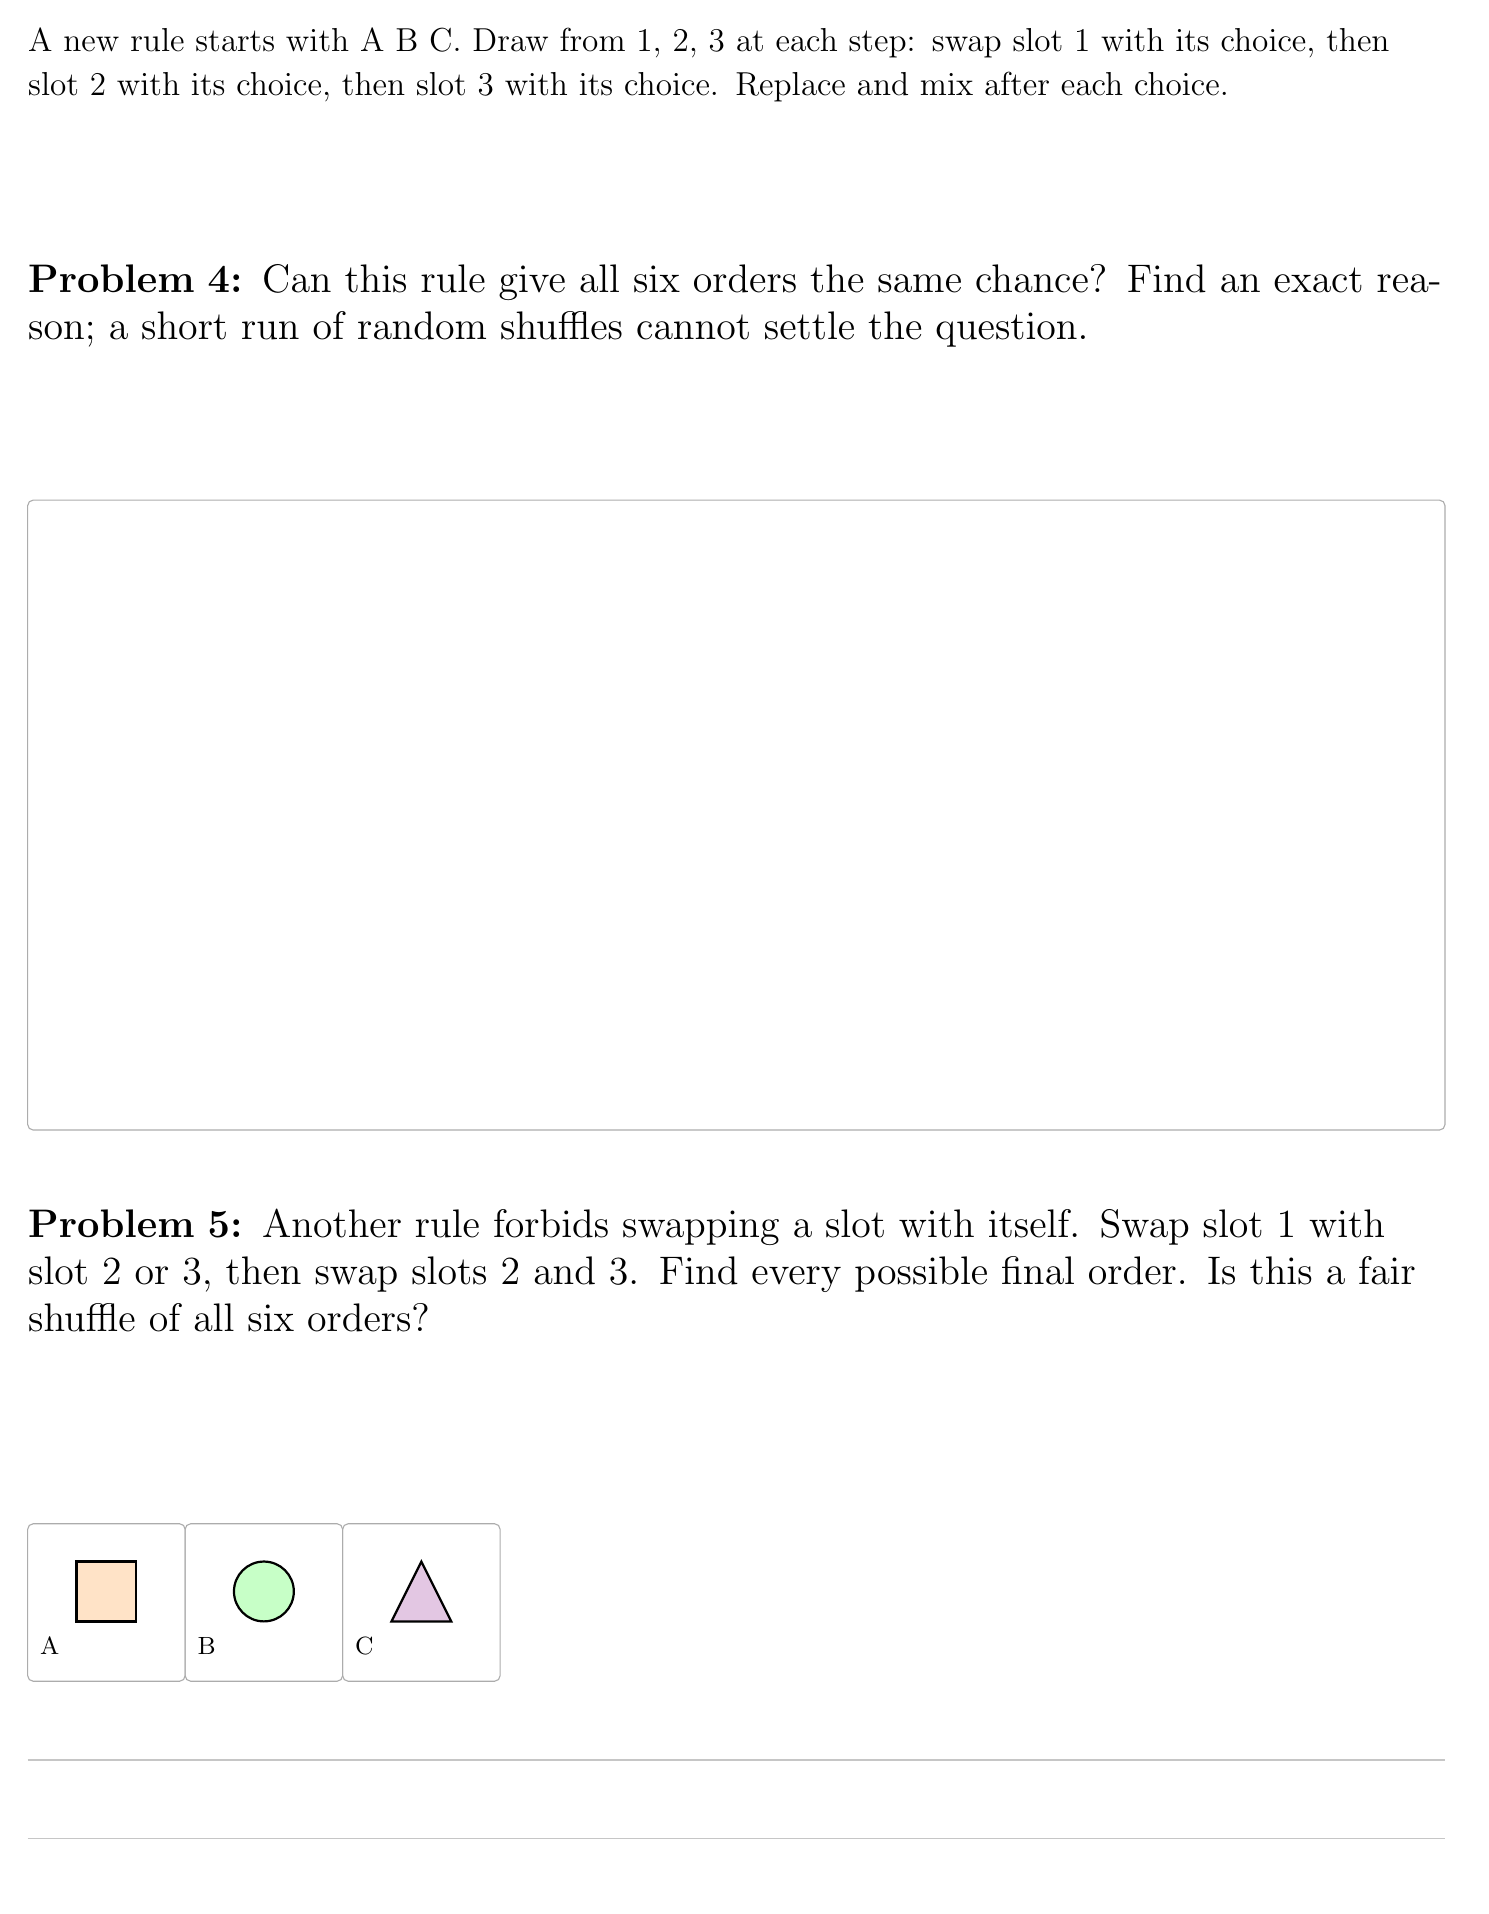
\begin{tikzpicture}[x=1cm,y=1cm]\path[use as bounding box] (0,0) rectangle (18.2,-23.6);
\node[anchor=north west,text width=18cm,inner sep=0pt,font=\fontsize{13}{16}\selectfont] at (0,0) {A new rule starts with A B C. Draw from 1, 2, 3 at each step: swap slot 1 with its choice, then slot 2 with its choice, then slot 3 with its choice. Replace and mix after each choice.};
\node[anchor=north west,text width=18cm,inner sep=0pt,font=\fontsize{14}{17}\selectfont] at (0,-3) {\textbf{Problem 4:} Can this rule give all six orders the same chance? Find an exact reason; a short run of random shuffles cannot settle the question.};
\draw[gray!65,rounded corners=2pt] (0,-6) rectangle (18,-14);
\node[anchor=north west,text width=18cm,inner sep=0pt,font=\fontsize{14}{17}\selectfont] at (0,-15) {\textbf{Problem 5:} Another rule forbids swapping a slot with itself. Swap slot 1 with slot 2 or 3, then swap slots 2 and 3. Find every possible final order. Is this a fair shuffle of all six orders?};
\draw[gray!65,rounded corners=2pt] (0.0,-19) rectangle (2.0,-21);
\draw[fill=orange!22,line width=.8pt] (0.62,-20.24) rectangle (1.38,-19.48);
\node[anchor=north west,text width=1.8cm,inner sep=0pt,font=\fontsize{9}{12}\selectfont] at (0.15,-20.44) {A};
\draw[gray!65,rounded corners=2pt] (2.0,-19) rectangle (4.0,-21);
\draw[fill=green!22,line width=.8pt] (3.0,-19.86) circle (0.38);
\node[anchor=north west,text width=1.8cm,inner sep=0pt,font=\fontsize{9}{12}\selectfont] at (2.15,-20.44) {B};
\draw[gray!65,rounded corners=2pt] (4.0,-19) rectangle (6.0,-21);
\draw[fill=violet!22,line width=.8pt] (5.0,-19.48) -- (5.38,-20.24) -- (4.62,-20.24) -- cycle;
\node[anchor=north west,text width=1.8cm,inner sep=0pt,font=\fontsize{9}{12}\selectfont] at (4.15,-20.44) {C};
\draw[gray!45] (0,-22) -- (18,-22);
\draw[gray!45] (0,-23) -- (18,-23);
\end{tikzpicture}
\newpage
\noindent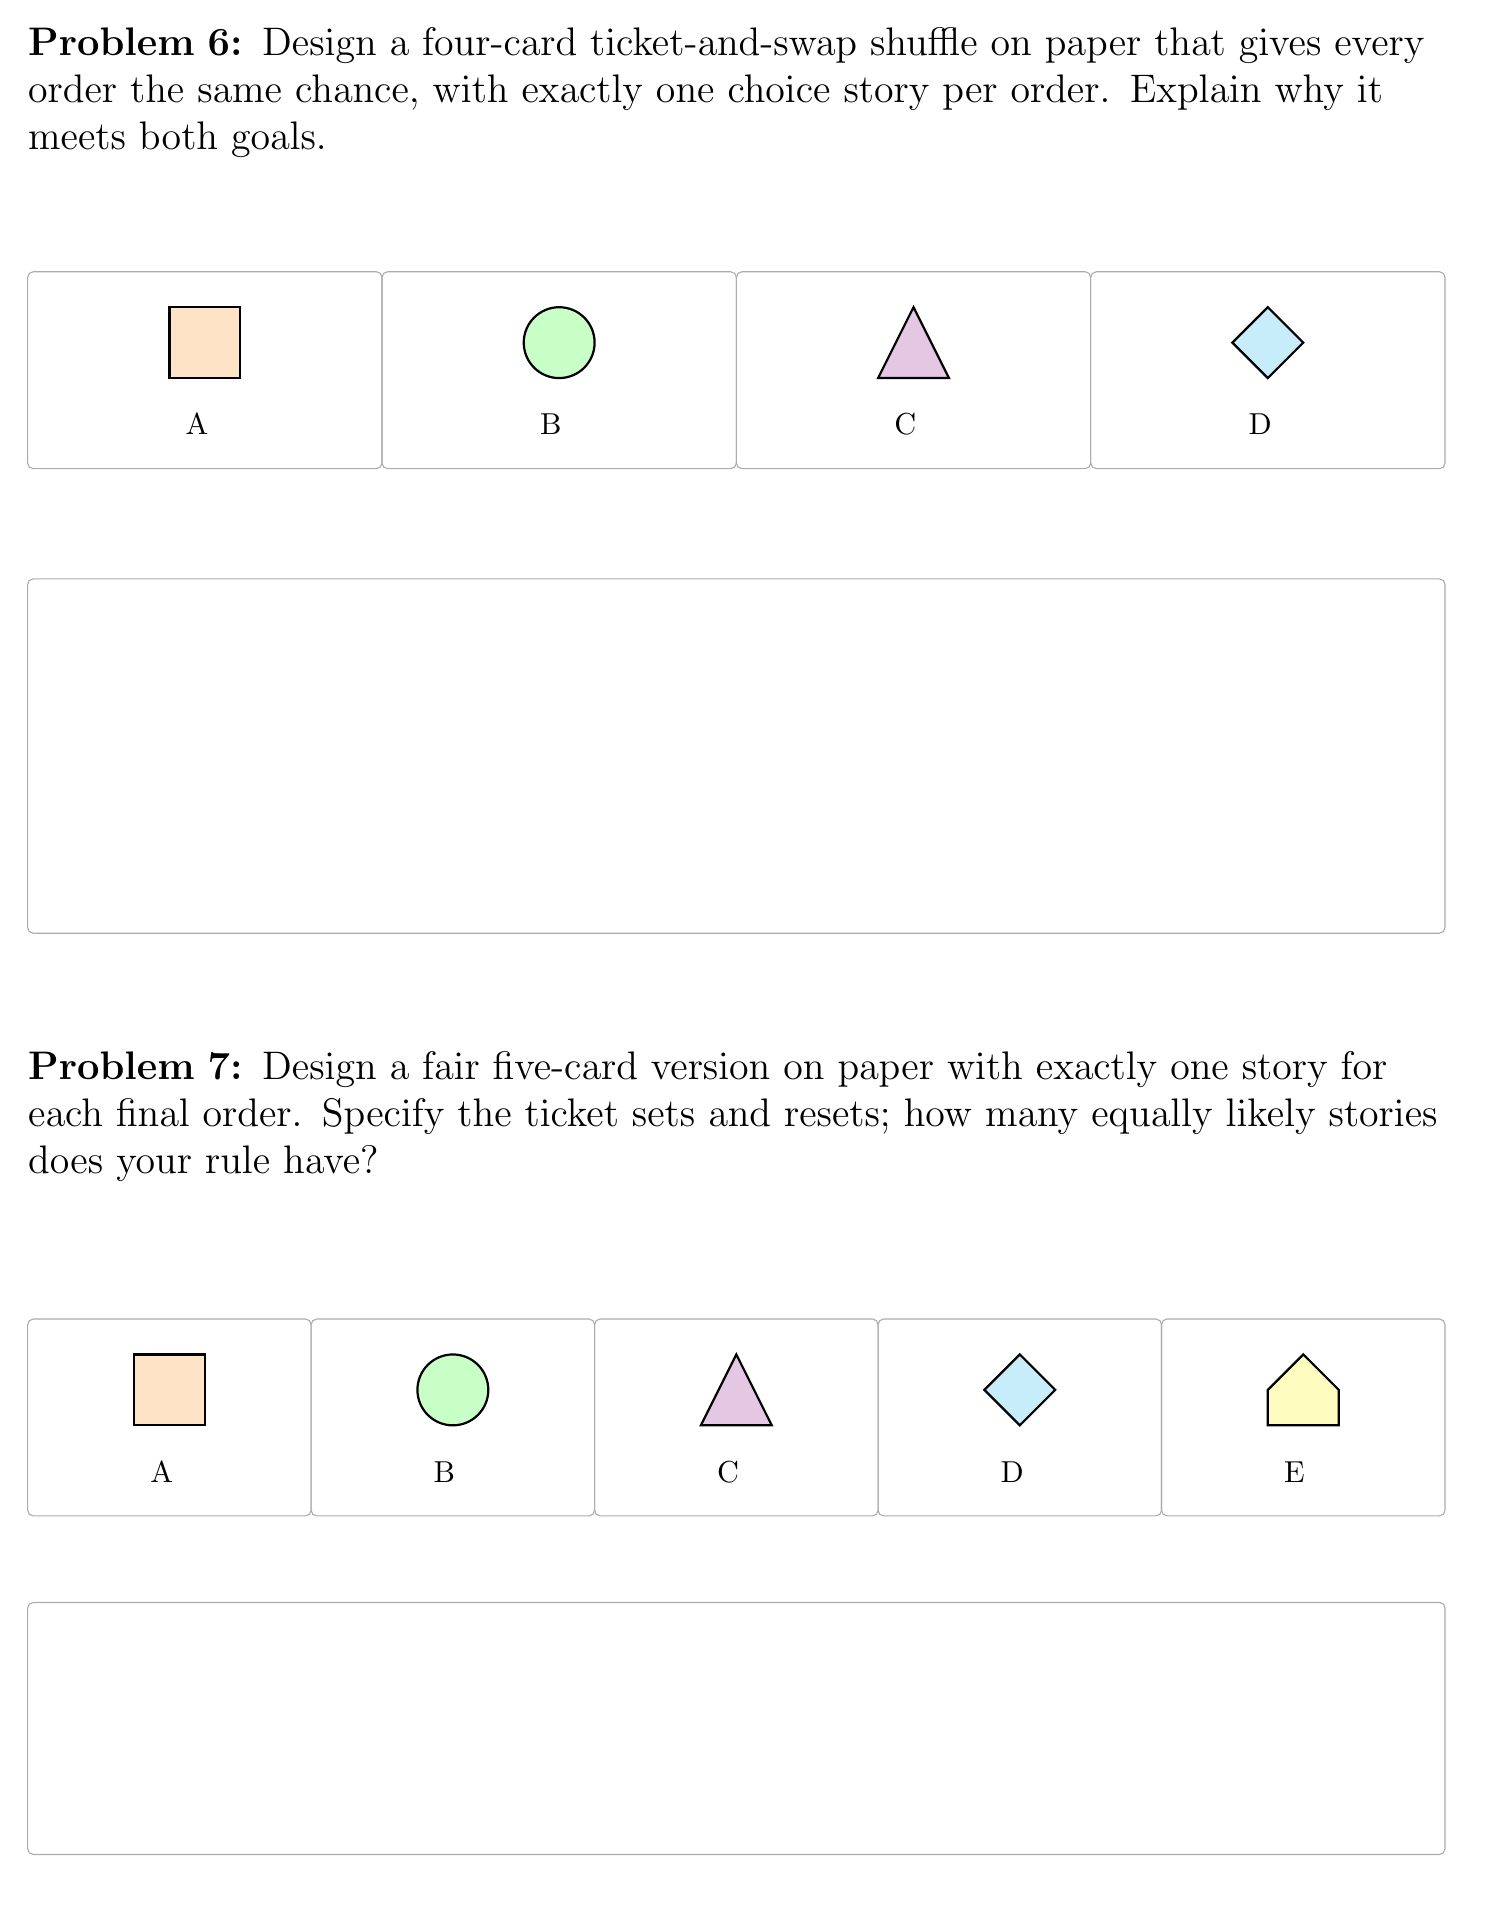
\begin{tikzpicture}[x=1cm,y=1cm]\path[use as bounding box] (0,0) rectangle (18.2,-23.6);
\node[anchor=north west,text width=18cm,inner sep=0pt,font=\fontsize{14}{17}\selectfont] at (0,0) {\textbf{Problem 6:} Design a four-card ticket-and-swap shuffle on paper that gives every order the same chance, with exactly one choice story per order. Explain why it meets both goals.};
\draw[gray!65,rounded corners=2pt] (0.0,-3.1) rectangle (4.5,-5.6);
\draw[fill=orange!22,line width=.8pt] (1.8,-4.45) rectangle (2.7,-3.55);
\node[anchor=north west,text width=0.8cm,inner sep=0pt,font=\fontsize{11}{14}\selectfont] at (2.0,-4.9) {A};
\draw[gray!65,rounded corners=2pt] (4.5,-3.1) rectangle (9.0,-5.6);
\draw[fill=green!22,line width=.8pt] (6.75,-4) circle (0.45);
\node[anchor=north west,text width=0.8cm,inner sep=0pt,font=\fontsize{11}{14}\selectfont] at (6.5,-4.9) {B};
\draw[gray!65,rounded corners=2pt] (9.0,-3.1) rectangle (13.5,-5.6);
\draw[fill=violet!22,line width=.8pt] (11.25,-3.55) -- (11.7,-4.45) -- (10.8,-4.45) -- cycle;
\node[anchor=north west,text width=0.8cm,inner sep=0pt,font=\fontsize{11}{14}\selectfont] at (11.0,-4.9) {C};
\draw[gray!65,rounded corners=2pt] (13.5,-3.1) rectangle (18.0,-5.6);
\draw[fill=cyan!22,line width=.8pt] (15.75,-3.55) -- (16.2,-4) -- (15.75,-4.45) -- (15.3,-4) -- cycle;
\node[anchor=north west,text width=0.8cm,inner sep=0pt,font=\fontsize{11}{14}\selectfont] at (15.5,-4.9) {D};
\draw[gray!65,rounded corners=2pt] (0,-7) rectangle (18,-11.5);
\node[anchor=north west,text width=18cm,inner sep=0pt,font=\fontsize{14}{17}\selectfont] at (0,-13) {\textbf{Problem 7:} Design a fair five-card version on paper with exactly one story for each final order. Specify the ticket sets and resets; how many equally likely stories does your rule have?};
\draw[gray!65,rounded corners=2pt] (0.0,-16.4) rectangle (3.6,-18.9);
\draw[fill=orange!22,line width=.8pt] (1.35,-17.75) rectangle (2.25,-16.85);
\node[anchor=north west,text width=0.8cm,inner sep=0pt,font=\fontsize{11}{14}\selectfont] at (1.55,-18.2) {A};
\draw[gray!65,rounded corners=2pt] (3.6,-16.4) rectangle (7.2,-18.9);
\draw[fill=green!22,line width=.8pt] (5.4,-17.3) circle (0.45);
\node[anchor=north west,text width=0.8cm,inner sep=0pt,font=\fontsize{11}{14}\selectfont] at (5.15,-18.2) {B};
\draw[gray!65,rounded corners=2pt] (7.2,-16.4) rectangle (10.8,-18.9);
\draw[fill=violet!22,line width=.8pt] (9.0,-16.85) -- (9.45,-17.75) -- (8.55,-17.75) -- cycle;
\node[anchor=north west,text width=0.8cm,inner sep=0pt,font=\fontsize{11}{14}\selectfont] at (8.75,-18.2) {C};
\draw[gray!65,rounded corners=2pt] (10.8,-16.4) rectangle (14.4,-18.9);
\draw[fill=cyan!22,line width=.8pt] (12.600000000000001,-16.85) -- (13.05,-17.3) -- (12.600000000000001,-17.75) -- (12.150000000000002,-17.3) -- cycle;
\node[anchor=north west,text width=0.8cm,inner sep=0pt,font=\fontsize{11}{14}\selectfont] at (12.350000000000001,-18.2) {D};
\draw[gray!65,rounded corners=2pt] (14.4,-16.4) rectangle (18.0,-18.9);
\draw[fill=yellow!25,line width=.8pt] (15.75,-17.75) -- (16.65,-17.75) -- (16.65,-17.3) -- (16.2,-16.85) -- (15.75,-17.3) -- cycle;
\node[anchor=north west,text width=0.8cm,inner sep=0pt,font=\fontsize{11}{14}\selectfont] at (15.950000000000001,-18.2) {E};
\draw[gray!65,rounded corners=2pt] (0,-20) rectangle (18,-23.2);
\end{tikzpicture}
\end{document}
